\section*{Ejercicio 2}
\graphicspath{{Figuras/}}

Se procedió a aproximar la probabilidad $P(N)$ se obtener $N$ spikes en una dada realización. Para esto, obtuvo la cantidad de spikes total de cada una de las 128 realizaciones y se generó un histograma, el cual puede observarse en la Figura \ref{02:fig:Histograma}. 

\begin{figure}[h!]
    \centering
    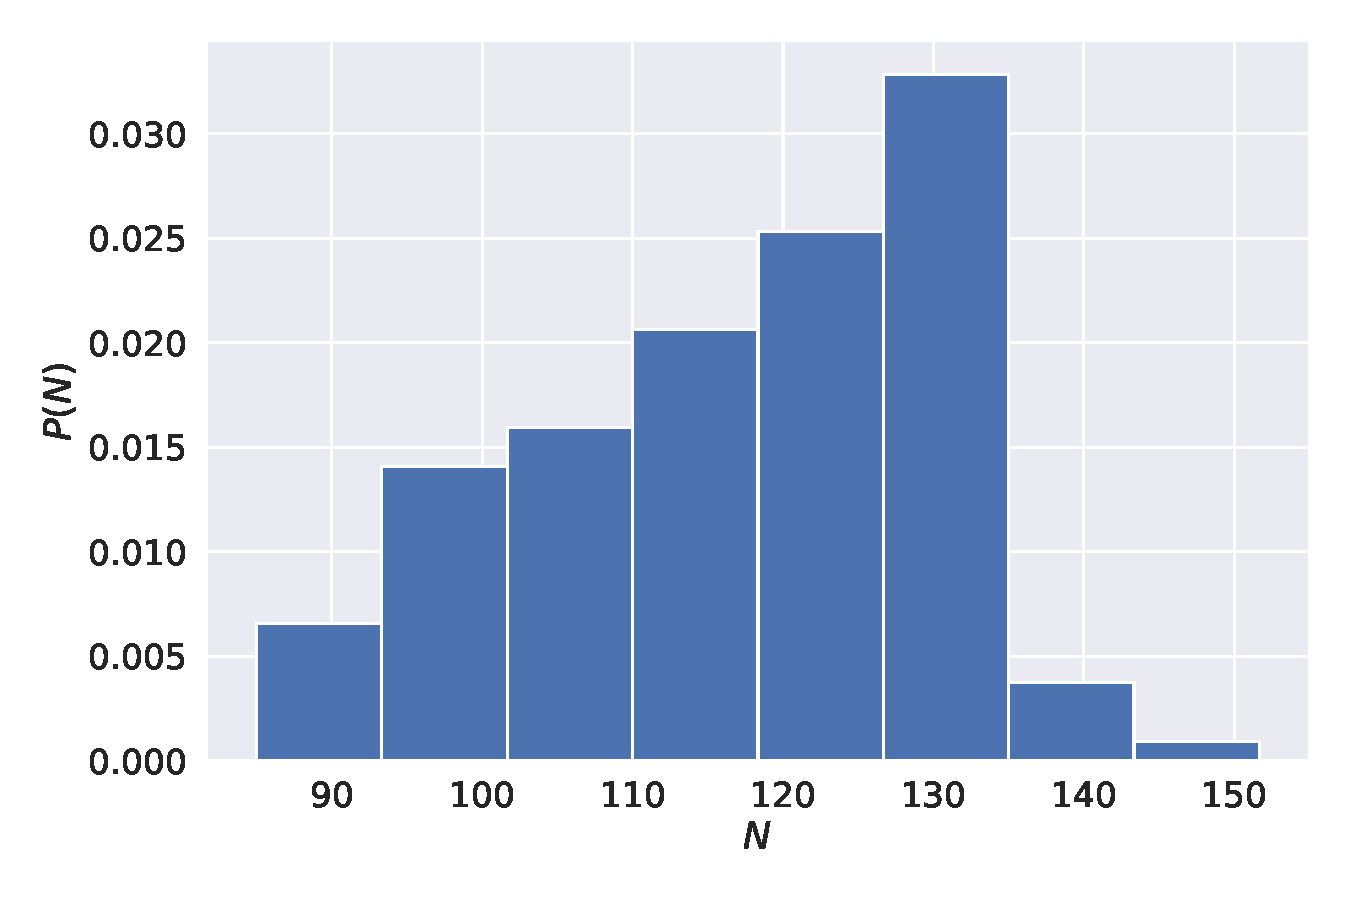
\includegraphics[width=0.75\textwidth]{2_PN.pdf}
    \caption{Histograma normalizado que aproxima la probabilidad $P(N)$ se obtener $N$ spikes en una dada realización.}
    \label{02:fig:Histograma}
\end{figure}

Luego se calculó el factor de Fano, el cual se obtiene como el cociente entre la desviación cuadrática y el valor medio de $P(N)$. Para el mismo se obtuvo $F\approx1.566$, lo cual es otra comprobación de que el proceso no es de Poisson. Por otro lado, en caso de ser un proceso de \textit{renewal}, debe verificarse que $F=CV^{2}$, pero $CV\approx0.432$, lo cual sugiere que la suposición de que es un proceso de \textit{renewal} tampoco es precisa.